\documentclass[a4 paper]{article}
% Set target color model to RGB



\usepackage[inner=2.0cm,outer=2.0cm,top=2.5cm,bottom=2.5cm]{geometry}
\usepackage{setspace}
\usepackage[rgb]{xcolor}
\usepackage{verbatim}
\usepackage{subcaption}
\usepackage{amsgen,amsmath,amstext,amsbsy,amsopn,tikz,amssymb,tkz-linknodes}
\usepackage{fancyhdr}
\usepackage[colorlinks=true, urlcolor=blue,  linkcolor=blue, citecolor=blue]{hyperref}
\usepackage[colorinlistoftodos]{todonotes}
\usepackage{rotating}
%\usetikzlibrary{through,backgrounds}

\usepackage{lmodern}
\usepackage[T1]{fontenc}
\usepackage[capposition=top]{floatrow}
\usepackage{hyperref}
\usepackage{graphicx}
\graphicspath{ {images/} }
\usepackage{booktabs}
\usepackage{changepage}
\usepackage{float}
\usepackage{fancyvrb}







\hypersetup{%
pdfauthor={Nick Korbit},%
pdftitle={Homework},%
%pdfkeywords={Tikz,latex,bootstrap,uncertaintes},%
pdfcreator={PDFLaTeX},%
pdfproducer={PDFLaTeX},%
}
%\usetikzlibrary{shadows}
% \usepackage[francais]{babel}
\usepackage{booktabs}


\newcommand{\ra}[1]{\renewcommand{\arraystretch}{#1}}

\newtheorem{thm}{Theorem}[section]
\newtheorem{prop}[thm]{Proposition}
\newtheorem{lem}[thm]{Lemma}
\newtheorem{cor}[thm]{Corollary}
\newtheorem{defn}[thm]{Definition}
\newtheorem{rem}[thm]{Remark}
\numberwithin{equation}{section}

\newcommand{\homework}[6]{
   \pagestyle{myheadings}
   \thispagestyle{plain}
   \newpage
   \setcounter{page}{1}
   \noindent
   \begin{center}
   \framebox{
      \vbox{\vspace{2mm}
    \hbox to 6.28in { {\bf ISYE 6420:~Bayesian Statistics \hfill {\small #2}} }
       \vspace{6mm}
       \hbox to 6.28in { {\Large \hfill #1  \hfill} }
       \vspace{6mm}
       \hbox to 6.28in { {\it Instructor: {\rm #3} \hfill Name: {\rm #5}, gtID: {\rm #6}} }
       %\hbox to 6.28in { {\it TA: #4  \hfill #6}}
      \vspace{2mm}}
   }
   \end{center}
   \markboth{#5 -- #1}{#5 -- #1}
   \vspace*{4mm}
}

\newcommand{\problem}[2]{~\\\fbox{\textbf{Problem #1}}\newline\newline}
\newcommand{\subproblem}[1]{~\newline\textbf{(#1)}}
\newcommand{\D}{\mathcal{D}}
\newcommand{\Hy}{\mathcal{H}}
\newcommand{\VS}{\textrm{VS}}
\newcommand{\solution}{~\newline\textbf{\textit{(Solution)}} }

\newcommand{\bbF}{\mathbb{F}}
\newcommand{\bbX}{\mathbb{X}}
\newcommand{\bI}{\mathbf{I}}
\newcommand{\bX}{\mathbf{X}}
\newcommand{\bY}{\mathbf{Y}}
\newcommand{\bepsilon}{\boldsymbol{\epsilon}}
\newcommand{\balpha}{\boldsymbol{\alpha}}
\newcommand{\bbeta}{\boldsymbol{\beta}}
\newcommand{\0}{\mathbf{0}}



%%%%%%%%%%%%%%%%%%%%%%%%%%%%%%%%%%%%%%%%
%%			 Document				  %%
%%%%%%%%%%%%%%%%%%%%%%%%%%%%%%%%%%%%%%%%


\begin{document}
	
\homework{Homework \#5}{Spring 2020}{Roshan Vengazhiyil, Brani Vidakovic}{}{Nick Korbit}{903263968}


%%%%%%%%%%%%%%%%%%%%%%%%%%%%%%%%%%%%%%%%
%%			 Problem 1				  %%
%%%%%%%%%%%%%%%%%%%%%%%%%%%%%%%%%%%%%%%%

\problem{1}

Let $x$ be the total blood volume
of normal newborn babies in
whom the cord was clamped early. We
then define $y$ as the total blood volume
of normal newborn babies in whom the cord 
was not clamped until the placenta 
began to descend. We model $x$ and $y$ as
Gamma with non-informative $(0.01, 0.01)$
priors:

\begin{align*}
x	\sim\mathcal{G}a\left(a_{x},b_{x}\right) \\
y	\sim\mathcal{G}a\left(a_{y},b_{y}\right) \\
a_{x},b_{x},a_{y},b_{y}	\sim\mathcal{G}a\left(0.001,0.001\right)
\end{align*}

Given observed 16 data points we 
specify an OpenBUGS model as

\begin{Verbatim}
for (i in 1:n) {
	x[i] ~ dgamma(a_x, b_x)
	y[i] ~ dgamma(a_y, b_y)
}
	
a_x ~ dgamma(0.001, 0.001)
b_x ~ dgamma(0.001, 0.001)
a_y ~ dgamma(0.001, 0.001)
b_y ~ dgamma(0.001, 0.001)
\end{Verbatim} 

We also know that the mean of Gamma is $\alpha/\beta$,
so we add calculation of means and their difference
to the model:

\begin{Verbatim}
mean_x <- a_x/b_x
mean_y <- a_y/b_y
diff <- mean_x - mean_y
\end{Verbatim} 

We initialize values for the priors as ones:
\begin{Verbatim}
list(a_x=1, b_x=1, a_y=1, b_y=1)  
\end{Verbatim} 



Let's now run an OpenBUGS simulation. We burn
the first 10000 observation and update the model 
with the next 100000 samples. First, we plot 
densities for means and their difference:

\begin{figure}[H]
	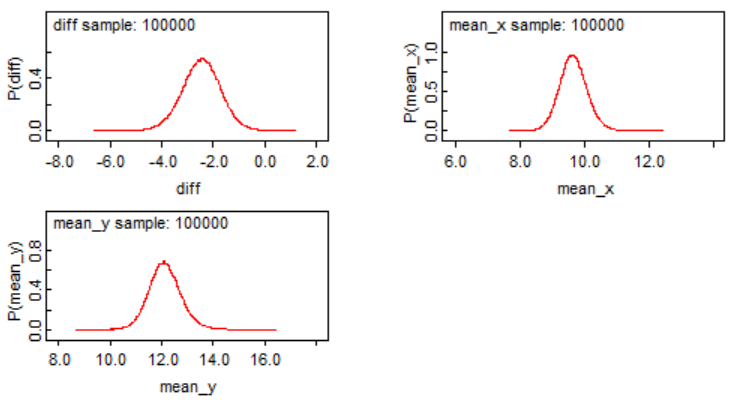
\includegraphics[scale=1.0]{q1}
	\centering
	%	\caption{cdf .}
	\label{q1}
\end{figure}

We notice that visually the difference is far 
from $0$ and the means themselves are very 
different. Let's see the statistics for 
the observed variables.

\begin{figure}[H]
	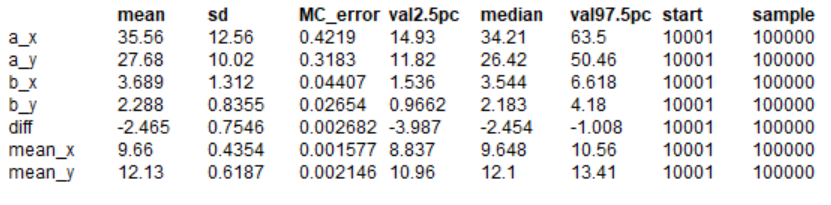
\includegraphics[scale=1.0]{q1_2}
	\centering
	%	\caption{cdf .}
	\label{q1_2}
\end{figure}


The 95\% credible set for the difference 
in means is $(-3.987, -1.008)$, so that
 $0$ is outside the set. \\

\textbf{Note}: the full OpenBUGS code is available 
at \textit{babies0.odc} in the attached archive.

 




%%%%%%%%%%%%%%%%%%%%%%%%%%%%%%%%%%%%%%%%
%%			 Problem 2				  %%
%%%%%%%%%%%%%%%%%%%%%%%%%%%%%%%%%%%%%%%%

\problem{2}

Let $y$ be the variable we would like to 
predict -- geographic location of wolves.
We model $y$ as

\begin{align*}
	y_{i}	\sim\mathcal{B}er\left(p_{i}\right) \\
	logit\left(p_{i}\right)	=\log\frac{p_{i}}{1-p_{i}}=\alpha+\beta_{gender}x_{gender}+\beta_{x3}x_{3}+\beta_{x7}x_{7}
\end{align*}

For each of the coefficients we set a 
normal prior with $\mu=0$ and $precision=0.01$. 
So that the OpenBUGS model is 

\begin{Verbatim}
# Training
for (i in 1:n) {
	logit(p[i]) <- alpha + b.gender*gender[i] + b.x3*x3[i] + b.x7*x7[i]
	arctic[i] ~ dbern(p[i])
}

alpha ~ dnorm(0.0, 0.01)
b.gender ~ dnorm(0.0, 0.01)
b.x3 ~ dnorm(0.0, 0.01)
b.x7 ~ dnorm(0.0, 0.01)
\end{Verbatim} 

We specify the initial values as $1$ for $\alpha$ 
and zeros for other coefficients:
\begin{Verbatim}
list(alpha=1, b.gender=0, b.x3=0, b.x7=0)  
\end{Verbatim} 


Knowning the characteristics 
of the new observation we proceed with inference:
\begin{Verbatim}
# Inference
logit(p_new) <- alpha + b.gender*xgender + b.x3*xx3 + b.x7*xx7

DATA
list(n=25, xx3=5.28, xx7=1.78, xgender=1) 
\end{Verbatim} 

Let's now run an OpenBUGS simulation. We start 
with burning 
the first 10000 observation and update the model 
with the next 100000 samples. First, we plot 
density for the new point $p_{new}$:

\begin{figure}[H]
	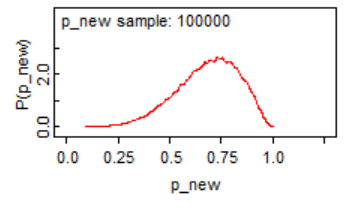
\includegraphics[scale=1.0]{q2}
	\centering
	%	\caption{cdf .}
	\label{q2}
\end{figure}

We notice that visually the prediction
is more skewed towards $y=1$ -- the Arctic location.
Let's investigate statistics:

\begin{figure}[H]
	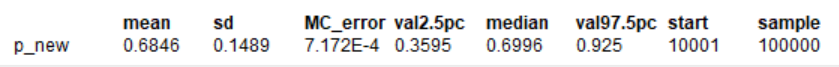
\includegraphics[scale=1.0]{q2_2}
	\centering
	\label{q2_2}
\end{figure}

The mean of the posterior (our Bayes estimator)
is $0.6846$, so that we conclude that with 
probability $p=0.6846$ our new observation 
point belongs to the Arctic location ($y=1$).
Notice also the relatively large 95\% credible set 
bounds -- $(0.3595, 0.925)$. So we cannot 
safely assume that the new point is from the Arctic. \\


\textbf{Note}: the full OpenBUGS code is available 
at \textit{wolves0.odc} in the attached archive.


%%%%%%%%%%%%%%%%%%%%%%%%%%%%%%%%%%%%%%%%
%%			 Problem 3				  %%
%%%%%%%%%%%%%%%%%%%%%%%%%%%%%%%%%%%%%%%%

\problem{3}

Let's define $y$ as the number of micronuclei
and $x$ as the dose (in Gy). We model 
$y$ as a Poisson regression:

\begin{align*}
	y_{i} & \sim\mathcal{P}oi\left(\lambda_{i}\right)\\
	\log\left(\lambda_{i}\right) & =\beta_{0}+\beta_{1}x_{i}
\end{align*}


For each of the coefficients we set a 
normal prior with $\mu=0$ and $precision=0.01$. 
So that the OpenBUGS model is 

\begin{Verbatim}
# Training
for (i in 1:n)
{
	y[i] ~ dpois(lambda[i])
	lambda[i] <- exp(beta0 + beta1 * x[i])
}

beta0 ~ dnorm(0, 0.01)
beta1 ~ dnorm(0, 0.01)
\end{Verbatim} 


Knowning the characteristics 
of the new observation we proceed with inference:
\begin{Verbatim}
# Inference
lambda_new <- exp(beta0 + beta1 * xdose)
y_new ~ dpois(lambda_new)
}

DATA
list(n=6000,  xdose=3.5)
\end{Verbatim} 

Let's now run an OpenBUGS simulation. We start 
with burning 
the first 500 observation and update the model 
with the next 3000 samples. First, we plot 
density for the new point $y_{new}$:

\begin{figure}[H]
	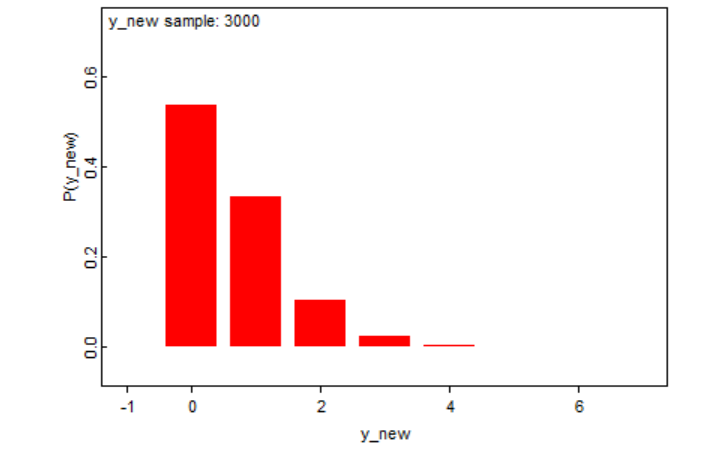
\includegraphics[scale=0.9]{q3}
	\centering
	\label{q3}
\end{figure}

We notice that the probability mass is skewed towards
$n=0$ and $n=1$ for dose of $3.5$ Gy.

Let's investidate statistics.

\begin{figure}[H]
	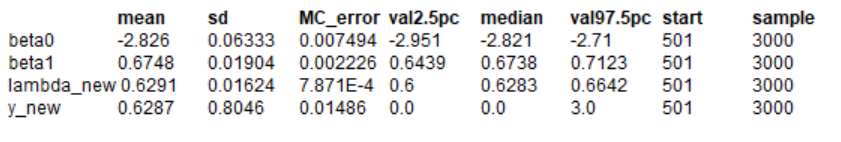
\includegraphics[scale=1.0]{q3_2}
	\centering
	\label{q3_2}
\end{figure}

We conclude that the average number 
of micronuclei for dose of 3.5 Gy 
is 0.6287. That's our Bayes estimator (the mean 
of the posterior distribution). \\


\textbf{Note}: the full OpenBUGS code is available 
at \textit{micronuclei0.odc} in the attached archive.


%%%%%%%%%%%%%%%%%%%%%%%%%%%%%%%%%%%%%%%%
%%			 Bibliography			  %%
%%%%%%%%%%%%%%%%%%%%%%%%%%%%%%%%%%%%%%%%

\begin{thebibliography}{9}


\bibitem{stat}\label{stat} 
Engineering Biostatistics: An Introduction using MATLAB and WinBUGS. 
Brani Vidakovic - Wiley Series in Probability and Statistics.

\end{thebibliography}



\end{document} 